
\section{Problem 2}
\label{part2}
Write a Python program that:
\begin{enumerate} 
\item takes one argument, like "Old Dominion" or "Virginia Tech" 
\item takes another argument specified in seconds (e.g., "60" for one minute).
\item takes a URI as a third argument:\\
\url{http://sports.yahoo.com/college-football/scoreboard/}\\
or\\
\url{http://sports.yahoo.com/college-football/scoreboard/?week=2\&conf=all}\\
or\\
\url{ http://sports.yahoo.com/college-football/scoreboard/?week=1\&conf=72}\\
etc.\\
\item dereferences the URI, finds the game corresponding to the team
     argument, prints out the current score (e.g., "Old Dominion 27, 
     East Carolina 17), sleeps for the specified seconds, and then
     repeats (until control-C is hit).
\end{enumerate}

\subsection{Solution}
\begin{enumerate}
\item In order to write this program firstly the source code for the URL should be examined.
\item Find elements in the html code where the team names and scores are located by using "urllib2.urlopen()" function imported from "urllib2" library .check for the div where all the content we want is located and note down the element names
\item Extract the part of code we are looking for by using "BeautifulSoup" library. 
\item The 'div' that had score of a teams are read and stored in to a new array 
\item Get the Team name as a Argument 1 and sleep time as an Argument 2 from a command line argument.
\item Now looping the stored array, check for the desired team name in the array and get the score associated to the team. 
\item By using the sleep method, the program does not exit till the control-C is hit, as the sleep time is given the program keeps updating the result for the given time.
\end{enumerate}

\subsection{Results}
\begin{enumerate}
\item To get the result the below command should be executed 
\begin{verbatim}
retrieve_american_football.py "arizona" 5 \
"http://sports.yahoo.com/college-football/scoreboard/?week=2&conf=all"
\end{verbatim}
\end{enumerate}
\begin{figure}[ht]    
    \begin{center}
        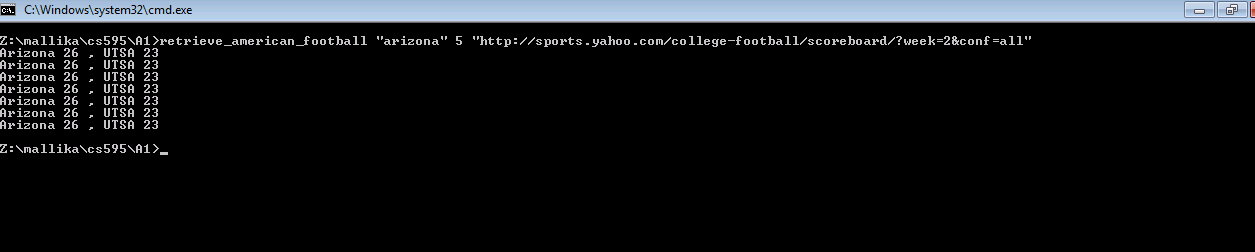
\includegraphics[scale=0.45]{part2-result.png}
        \caption{Sample Output}
        \label{fig:X-distribution}
    \end{center}
\end{figure}

\subsection{Code Listing}
\lstinputlisting[language=Python, breaklines=true]{retrieve_american_football.py}